\setcounter{secnumdepth}{2}
\section{Giới thiệu}

\subsection{Bảng phân công và đánh giá tiến độ công việc}
Dưới đây là bảng phân công và đánh giá tiến độ công việc của nhóm:

\begin{center}
	\begin{tabular}{|c|c|c|}
		\hline
		\textbf{Họ và tên} & \textbf{Các công việc phụ trách} & \textbf{Tiến độ công việc} \\ \hline
		\multirow{3}{*}{Nguyễn Tấn Duy Anh} & Cài đặt thuật toán BFS & 100\% \\ \cline{2-3} 
		& \multirow{2}{*}{\begin{tabular}[c]{@{}c@{}} Viết giới thiệu trò chơi\\ và thuật toán BFS \end{tabular}} & \multirow{2}{*}{100\%} \\
		&  &  \\ \hline
		\multirow{3}{*}{Bùi Hồng Phúc} & Cài đặt thuật toán DFS & 100\% \\ \cline{2-3} 
		& Thiết kế giao diện chương trình & 100\% \\ \cline{2-3}
		& Viết thuật toán DFS & 100\% \\ \hline
		\multirow{3}{*}{Nguyễn Lê Anh Phúc} & Cài đặt thuật toán A* & 100\% \\ \cline{2-3} 
		& Kiểm thử chương trình & 100\% \\ \cline{2-3}
		& Viết thuật toán A* & 100\% \\ \hline
		\multirow{3}{*}{Hồ Minh Quang} & Cài đặt thuật toán UCS & 100\% \\ \cline{2-3} 
		& Viết toàn bộ khung báo cáo \LaTeX & 100\% \\ \cline{2-3}
		& Viết thuật toán UCS & 100\% \\ \hline
	\end{tabular}
\end{center}

\subsection{Bài toán tìm kiếm}
Bài toán tìm kiếm là một trong những bài toán phổ biến trên nhiều lĩnh vực khác nhau với mục tiêu là tìm một cấu trúc "$Y$" (gọi là \emph{lời giải}) trong một thực thể "$X$" nào đó. Một vài ví dụ về bài toán tìm kiếm có thể kể đến như: truy vấn thông tin trên cơ sở dữ liệu, giải đố mê cung, tìm đường đi, ... \cite{search-wiki} \cite{search-brit}

Một bài toán tìm kiếm có thể được biểu diễn như sau: \cite{AI_HCMUS}
\begin{itemize}[labelindent=2em, labelsep=0.3cm, leftmargin=1cm, wide=\parindent, topsep=0.1cm, itemsep=-1ex, partopsep=1.5ex, parsep=1.5ex]
	\item \textbf{Không gian trạng thái:} Đây là thành phần chứa toàn bộ các trạng thái mà bài toán có thể phát sinh.
	\item \textbf{Trạng thái ban đầu:} Đây là điểm xuất phát của bài toán tìm kiếm.
	\item \textbf{Hàm trạng thái con:} Đây là hàm phát sinh trạng thái mới từ một trạng thái cụ thể $x$. Hàm này cùng với trạng thái ban đầu tạo nên không gian trạng thái cho bài toán.
	\item \textbf{Tập hợp trạng thái đích:} Đây là tập hợp con của không gian trạng thái, chứa các trạng thái để kết thúc bài toán. Bài toán kết thúc khi đạt được một hoặc nhiều trạng thái đích khác nhau trong tập hợp này, tùy theo ngữ cảnh của bài toán.
	\item \textbf{Hàm tính chi phí:} Đây là hàm tính toàn bộ chi phí đường đi cho lời giải của bài toán.
\end{itemize}

Các thuật toán tìm kiếm có thể được phân thành hai loại thuật toán: \emph{Tìm kiếm không có thông tin} (Tìm kiếm ``mù'') và \emph{Tìm kiếm có thông tin} (Tìm kiếm ``tối ưu''). Dưới đây là một số đặc trưng và so sánh giữa hai loại thuật toán:

\begin{center}
	\begin{tabular}{|l|c|c|}
		\hline
		 \textbf{Loại thuật toán} & \textbf{Tìm kiếm ``mù''} & \textbf{Tìm kiếm ``tối ưu''} \\ \hline
		 \textbf{Hiệu suất} & Chậm hơn do không có thông tin & Nhanh hơn \\ \hline
		 \multirow{2}{*}{\textbf{Tính xác định}} & \multirow{2}{*}{Luôn có kết quả} & Có thể có kết quả \\
		 & & hoặc không \\ \hline
		 \multirow{2}{*}{\textbf{Thời gian}} & \multirow{2}{*}{Thời gian chạy chậm hơn} & Thời gian chạy nhanh hơn \\
		 & & do có hàm tối ưu \\ \hline
		 \multirow{2}{*}{\textbf{Bộ nhớ}} & \multirow{2}{*}{Sử dụng nhiều bộ nhớ hơn} & Sử dụng bộ nhớ ít hơn do \\
		 & & sử dụng hàm tối ưu \\ \hline
		 \multirow{2}{*}{\textbf{Phạm vi}} & \multirow{2}{*}{Phạm vi tìm kiếm lớn do} & Phạm vi tìm kiếm nhỏ \\
		 \multirow{2}{*}{\textbf{tìm kiếm}} & \multirow{2}{*}{không loại bỏ trạng thái xấu} & nhờ loại bỏ trạng thái xấu \\
		  & & thông qua hàm tối ưu \\ \hline
		  & Tìm kiếm theo chiều sâu & Tìm kiếm tham lam \\
		  & (Depth-first search/DFS) & (Greedy search) \\
		 \textbf{Một số} & Tìm kiếm theo chiều rộng & Tìm kiếm leo đồi \\
		 \textbf{thuật toán} & (Breadth-first search/BFS) & (Hill-climbing search) \\
		  & Tìm kiếm đồng nhất chi phí & \multirow{2}{*}{Tìm kiếm A*} \\
		  & (Uniform-cost search/UCS) & \\ \hline
	\end{tabular}
\end{center}

Bài toán tìm kiếm được đề cập trong báo cáo này là giải đố trò chơi Sokoban.

\subsection{Trò chơi Sokoban}
Sokoban là một trò chơi giải đố với mục tiêu là phải đẩy các thùng hàng trong kho vào các vị trí lưu trữ. Trò chơi này được thiết kế vào năm 1981 bởi Hiroyuki Imabayashi và ra mắt công chúng lần đầu vào tháng 12 năm 1982 bởi công ty Thinking Rabbit tại Takarazuka, Nhật Bản. \cite{sokoban-wiki}

\begin{figure}[htp!]
	\centering
	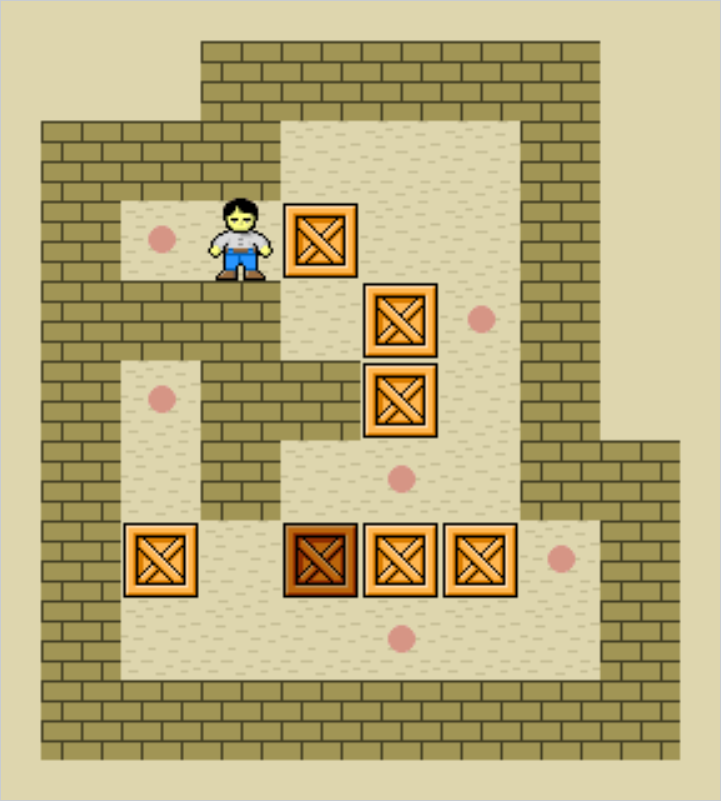
\includegraphics[width = 0.5\textwidth]{Sokoban}
	\caption[Hình ảnh một màn chơi của Sokoban]{Hình ảnh một màn chơi của Sokoban (Nguồn: )}
\end{figure}
% \protect{\hypersetup{urlcolor=blue}\href{https://en.wikipedia.org/wiki/Sokoban#/media/File:Sokoban_ani.gif}{Wikipedia}}

\underline{\textbf{Mô tả trò chơi:}} Nhà kho chứa các thùng hàng được biểu diễn bằng các ô trên bản đồ, mỗi ô biểu diễn một phần sàn hoặc tường của nhà kho. Một số ô sàn chứa các thùng hàng, một số khác là các vị trí lưu trữ. Người chơi chỉ có thể đẩy một thùng hàng khi đứng sát bên thùng hàng đó và không có tường hoặc thùng hàng khác chặn đường. \linebreak Màn chơi hoàn thành khi tất cả các thùng hàng đều được đẩy vào vị trí lưu trữ.

\underline{\textbf{Những khó khăn có thể gặp:}} Trong quá trình diễn ra trò chơi, nếu đẩy các thùng hàng không cẩn thận thì người chơi có thể rơi vào trạng thái bế tắc (có ít nhất một thùng hàng không thể di chuyển được) khi gặp phải một trong các hình như dưới đây \cite{timo-sokoban}:

%Alternative citation
%@article{timo-sokoban,
%	author = {Virkkala, Timo},
%	title = {Solving Sokoban - Master Thesis},
%	date = {2011-04-12},
%	publisher = {University of Helsinki}
%}

\begin{figure}[htp!]
	\centering
	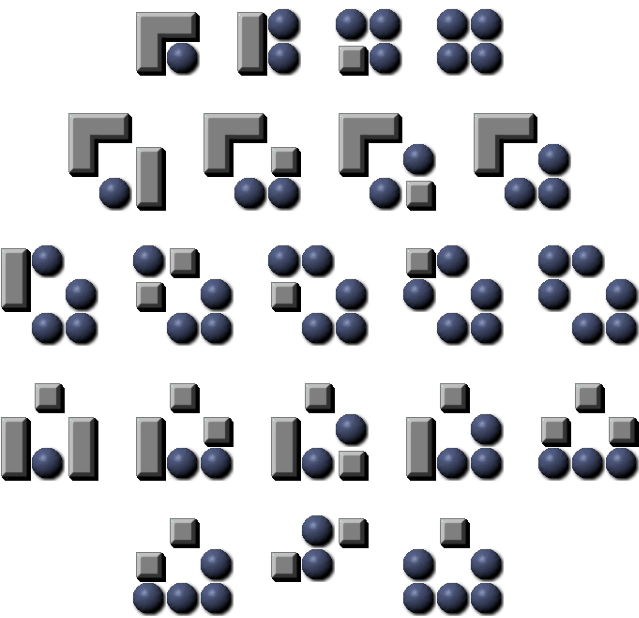
\includegraphics[width = 0.5\textwidth]{deadlock-patterns}
	\caption{Các hình có thể gặp trong trạng thái bế tắc}
	\label{fig:deadlocks}
\end{figure}

Vì thế, việc đẩy các thùng hàng cần phải được tính toán hết sức cẩn thận, trừ phi trạng thái bắt đầu chỉ có thể dẫn đến một trong các trạng thái bế tắc.

\subsection{Nội dung đồ án và chương trình của nhóm}

\subsubsection{Nội dung đồ án}
Nội dung của đồ án lần này là viết một chương trình để giải đố các màn chơi của Sokoban biến thể. Chủ đề của trò chơi là mê cung kho báu với các tảng đá được dùng để kích hoạt các công tắc trong mê cung để mở cánh cổng dẫn tới kho báu. Người chơi đóng vai một nhà thám hiểm trẻ với tham vọng tìm toàn bộ kho báu được ẩn giấu phía trong. Nhiệm vụ của người chơi là tìm ra một cách giải (nếu có) cho mê cung kho báu.

Điểm khác biệt rõ rệt của biến thể này so với trò chơi truyền thống là mỗi tảng đá đều có khối lượng. Điều này gợi thêm yêu cầu về tính tối ưu cho lời giải của bài toán.

\subsubsection{Chương trình giải của nhóm}
Nhóm đã viết một chương trình bằng ngôn ngữ Python để tìm lời giải cho mê cung kho báu bằng các thuật toán tìm kiếm trên đồ thị sau: Tìm kiếm theo chiều sâu (DFS); Tìm kiếm theo chiều rộng (BFS); Tìm kiếm đồng nhất chi phí (UCS); Tìm kiếm A*. Các thành phần của chương trình này bao gồm:
\begin{enumerate}[label=\bfseries\arabic*), labelindent=2em, labelsep=0.3cm, leftmargin=1cm, wide=\parindent, topsep=0.1cm, itemsep=-1ex, partopsep=1.5ex, parsep=1.5ex]
	\item \textbf{Lớp không gian trạng thái:} Toàn bộ không gian trạng thái được thiết lập bên trong tập tin \verb|maze.py|, gồm hai lớp đối tượng \verb|Node| và \verb|SearchSpace|.
	\begin{itemize}[labelindent=2em, labelsep=0.3cm, leftmargin=1cm, wide=1.5\parindent, topsep=0.1cm, itemsep=-1ex, partopsep=1.5ex, parsep=1.5ex]
		\item Lớp \verb|Node| được xây dựng để chứa một trạng thái (bộ hai biến \verb|(agent_pos;| \verb|stones_state_id)| đươc dùng để miêu tả một trạng thái, với \verb|agent_pos| là vị trí của người chơi và \verb|stone_state_id| là mã trạng thái trong danh sách các trạng thái của các tảng đá). Ngoài hai biến trên thì các biến \verb|prev_state, steps, weight| và \verb|move_label| lần lượt được dùng để lưu mã trạng thái đường đi trước đó, số bước di chuyển, khối lượng đá đã đẩy và ký tự đặc trưng cho hành động của người chơi.
		\item Lớp \verb|SearchSpace| được dùng để khởi tạo trò chơi cũng như lưu các trạng thái và tác vụ của người chơi. Biến \verb|stone_weights| được dùng để lưu khối lượng của từng tảng đá, \verb|stones_state_list| là một mảng lưu các trạng thái của các tảng đá trong màn chơi, với \verb|stones_state_list[0]| là trạng thái đầu tiên của chúng. Biến \verb|start| lưu vị trí ban đầu của người chơi, còn \verb|switches| là một mảng được dùng để lưu vị trí các công tắc trong mê cung.
		\item Ngoài ra, để phục vụ cho quá trình tìm kiếm, lớp \verb|SearchSpace| còn có biến \verb|row| để lưu số ô trong một dòng của màn chơi, biến \verb|column| để lưu số ô trong một cột, \verb|open_set| là một mảng lưu các \verb|Node| đang mở và \verb|closed_set| là mảng lưu các \verb|Node| đã đóng.
	\end{itemize}
	\item \textbf{Các bước đi của người chơi:} Lớp \verb|SearchSpace| có thiết lập các hàm tạo trạng thái mới từ các bước đi của người chơi, bao gồm:
	\begin{itemize}[labelindent=2em, labelsep=0.3cm, leftmargin=1cm, wide=1.5\parindent, topsep=0.1cm, itemsep=-1ex, partopsep=1.5ex, parsep=1.5ex]
		\item Kiểm tra nước đi cần thiết: Hàm \verb|isRedundant| được dùng để kiểm tra nếu trạng thái đang xét là không cần thiết. Có năm tính chất được dùng trong hàm này để kiểm tra, bao gồm: \verb|isLooped| được dùng để kiểm tra người chơi có đang đi trong một vòng lặp hay không, \verb|isAlternativeMove| được dùng để kiểm tra nếu trạng thái đã tồn tại trước đó, \verb|stoneInLoop| được dùng để kiểm tra nếu có một tảng đá bị đẩy ngược về một trạng thái trước đó, \verb|isDeadlocked| được dùng để kiểm tra nếu trạng thái đang xét là một trong bốn trạng thái bế tắc đầu tiên ở hình \ref{fig:deadlocks} và kiểm tra nếu người chơi di chuyển xa ra khỏi các tảng đá mà không gặp bất kỳ chướng ngại vật nào.
		\item Thao tác di chuyển của người chơi: Các hàm \verb|move_up, move_down, move_left,| \verb|move_right| được dùng để khởi tạo và kiểm tra hợp lệ của các trạng thái di chuyển lên, xuống, trái, phải của người chơi. \verb|move_label| tương ứng với các thao tác di chuyển trên lần lượt là \verb|u, d, l ,r|.
		\item Thao tác di chuyển một tảng đá của người chơi: Các hàm \verb|move_up, move_down,| \verb|move_left, move_right| được dùng để khởi tạo và kiểm tra hợp lệ của các trạng thái di chuyển một tảng đá lên, xuống, trái, phải của người chơi. \verb|move_label| tương ứng với các thao tác di chuyển trên lần lượt là \verb|U, D, L ,R|.
	\end{itemize}
	\item \textbf{Các thuật toán tìm kiếm:} Toàn bộ thuật toán tìm kiếm kể trên được miêu tả trong các hàm \verb|DFS, BFS, UCS| và \verb|AStar|. Chi tiết thuật toán sẽ được miêu tả ở các phần \ref{DFS}, \ref{BFS}, \ref{UCS} và \ref{AStar}. Đối với việc mở các trạng thái mới, lớp \verb|SearchSpace| có hỗ trợ hàm \verb|nodeExpansion| để mở các nước đi cần thiết và hợp lệ mới.
	\item \textbf{Giao diện:} Chương trình có giao diện đi kèm, giúp cho người dùng sử dụng chương trình dễ dàng cũng như biểu diễn đường đi của lời giải một cách trực quan hơn. Giao diện sẽ được biểu diễn ở phần \ref{tests-results}.
\end{enumerate}
\newpage
%\underline{\textbf{Một số hạn chế của chương trình:}} Do nhóm chưa tìm hiểu kĩ về ngôn ngữ lập trình Python cũng như các thư viện hỗ trợ, nên nhóm đã cài đặt các hàm trong một lớp, khiến cho thời gian chạy của chương trình khá dài do cơ chế truy xuất hàm trong một lớp của Python.
\subsubsection{Về mã giả và mã nguồn của các thuật toán}
Các thuật toán đều có cấu trúc mã nguồn khá tương tự nhau, do đó mã giả của chúng cũng sẽ tương tự nhau. Dưới đây là quy trình của một thuật toán tìm kiếm trong chương trình của nhóm:
\label{algo-struct}
\begin{enumerate}[label=\bfseries\arabic*), labelindent=2em, labelsep=0.3cm, leftmargin=1cm, wide=\parindent, topsep=0.1cm, itemsep=-1ex, partopsep=1.5ex, parsep=1.5ex]
	\item \textbf{Khởi tạo tập các trạng thái mở và thêm vị trí xuất phát:} Trong mã nguồn của nhóm, mảng \verb|open_set| trong lớp \verb|SearchSpace| đã khởi tạo một mảng với \verb|Node(start)| là phần tử đầu tiên. \verb|Node(start)| là đối tượng lưu trữ trạng thái đầu tiên của màn chơi.
	\item \textbf{Chọn một trạng thái đang mở và đóng nó lại}: Trong mã nguồn của nhóm, mảng \verb|closed_set| trong lớp \verb|SearchSpace| được dùng để lưu các trạng thái đã được đóng. Sau khi chọn được một trạng thái, trạng thái này sẽ được loại bỏ ra khỏi tập các trạng thái mở (\verb|open_set|) và thêm vào tập các trạng thái đóng (\verb|closed_set|). Tiêu chí chọn trạng thái tùy thuộc vào tính chất của thuật toán và sẽ được trình bày ở phần phía dưới.
	\item \textbf{Kiểm tra nếu trạng thái đích đã đóng:} Việc kiểm tra này sẽ cho biết nếu đã có một lời giải thỏa mãn. Dòng mã \verb|if goalReached(game.closed_set[-1])| sẽ đảm nhiệm việc này. Nếu chưa có trạng thái đích, thuật toán sẽ tiếp tục bước \textbf{4}. Ngược lại, thuật toán trả về một lời giải.
	\item \textbf{Mở các trạng thái mới từ trạng thái vừa đóng:} Việc mở các trạng thái mới sẽ tương ứng với các nước đi của người chơi trong trò chơi. Dòng mã \verb|new_nodes = game.nodeExpansion(...)| sẽ đảm nhiệm việc đóng trạng thái và mở các nước đi mới hợp lệ và cần thiết. Việc thêm trạng thái vào tập các trạng thái mở sẽ tùy thuộc vào thuật toán.
	\item \textbf{Kiểm tra nếu còn trạng thái mở:} Nếu không còn trạng thái nào được mở, kết thúc thuật toán. Ngược lại, thuật toán lặp lại từ bước \textbf{2}.
\end{enumerate}

\vskip 0.25 cm
Mã giả cho quy trình trên được biểu diễn như sau:

\vskip 0.125 cm
\textbf{thuật\_toán\_tìm\_kiếm}(màn\_chơi): \newline
\indent\indent tập\_mở $\gets$ [trạng\_thái\_đầu] \newline
\indent\indent tập\_đóng $\gets$ [] \newline
\indent\indent \textbf{khi} tập\_mở \textbf{còn trạng thái}: \newline
\indent\indent\indent trạng\_thái\_đóng\_mới $\gets$ \textbf{chọn\_trạng\_thái}(tiêu\_chí) \newline
\indent\indent\indent \textbf{thêm} trạng\_thái\_đóng\_mới \textbf{vào} tập\_đóng \newline
\indent\indent\indent \textbf{nếu} trạng\_thái\_đóng\_mới \textbf{là đích}: \newline
\indent\indent\indent\indent lời\_giải $\gets$ \textbf{biểu\_diễn\_lời\_giải}(trạng\_thái\_đóng\_mới) \newline
\indent\indent\indent\indent \textbf{trả về} lời\_giải \newline
\indent\indent\indent các\_trạng\_thái\_mới $\gets$ \textbf{mở\_rộng\_trạng\_thái}(trạng\_thái\_đóng\_mới) \newline
\indent\indent\indent \textbf{nếu có trạng thái trong}  các\_trạng\_thái\_mới: \newline
\indent\indent\indent\indent \textbf{thêm} các\_trạng\_thái\_mới \textbf{vào} tập\_mở \newline
\indent\indent\indent \textbf{nếu không có trạng thái trong} tập\_mở: \newline
\indent\indent\indent\indent \textbf{trả về} "Không có lời giải!" \newline

\newpage